\documentclass[border=3pt,tikz]{standalone}
\usepackage{tikz-3dplot}

\usetikzlibrary{arrows.meta} % for arrow size

\usetikzlibrary{decorations.pathreplacing}

\tikzset{arrowed/.style={decorate,
decoration={show path construction, 
moveto code={},
lineto code={
\draw[#1] (\tikzinputsegmentfirst) --  (\tikzinputsegmentlast);
},
curveto code={},
closepath code={},
}},arrowed/.default={-stealth}}
\usepackage{pgfplots}
\pgfplotsset{gradient function/.initial=f,
dx/.initial=0.01,dy/.initial=0.01}
\pgfmathdeclarefunction{xgrad}{2}{%
\begingroup%
\pgfkeys{/pgf/fpu,/pgf/fpu/output format=fixed}%
\edef\myfun{\pgfkeysvalueof{/pgfplots/gradient function}}%
\pgfmathparse{(\myfun(#1+\pgfkeysvalueof{/pgfplots/dx},#2)%
-\myfun(#1,#2))/\pgfkeysvalueof{/pgfplots/dx}}%
\pgfmathsmuggle\pgfmathresult\endgroup%
}%
\pgfmathdeclarefunction{ygrad}{2}{%
\begingroup%
\pgfkeys{/pgf/fpu,/pgf/fpu/output format=fixed}%
\edef\myfun{\pgfkeysvalueof{/pgfplots/gradient function}}%
\pgfmathparse{(\myfun(#1,#2+\pgfkeysvalueof{/pgfplots/dy})%
-\myfun(#1,#2))/\pgfkeysvalueof{/pgfplots/dy}}%
\pgfmathsmuggle\pgfmathresult\endgroup%
}%

\pgfplotsset{compat=1.17}

\begin{document}

\begin{figure}[!htbp]
  \resizebox{.6\textwidth}{!}{
    \begin{minipage}{0.6\textwidth}
      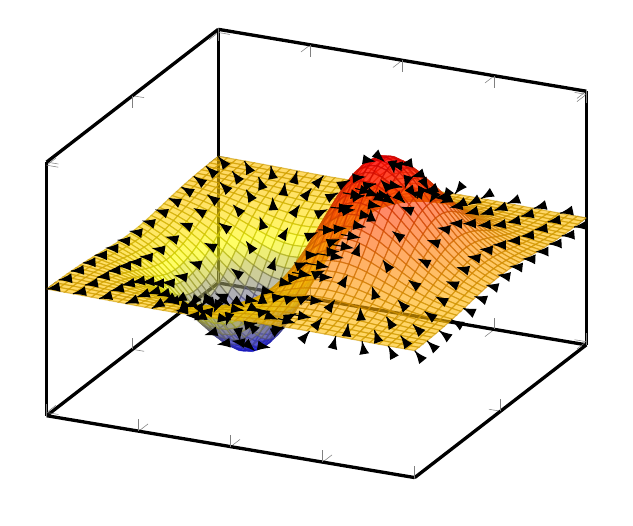
\begin{tikzpicture}
        \begin{axis}[
            domain=-2:2,
            axis line style ={very thick},
            xmin=-2, xmax=2,
            ymin=-2, ymax=2,
            yticklabel=\empty,
            xticklabel=\empty,
            zticklabel=\empty,
          ]
          \addplot3
          [surf,
            samples=42,
            opacity=0.6,
          ]
          {x/(0.01*exp(x^2+y^2))};
          \addplot3
          [black,
          quiver={
          u={(1-2*x^2)*exp(-x^2-y^2)},
          v={-2*x*y*exp(-x^2-y^2)},
          scale arrows=0.3,
          every arrow/.append style={%
          -{Latex[scale length={max(0.01,\pgfplotspointmetatransformed/1000)}]},
          },
          },
          samples=15]
          {x/(0.01*exp(x^2+y^2))};
        \end{axis}
      \end{tikzpicture}
    \end{minipage}
    \begin{minipage}{0.3\textwidth}

      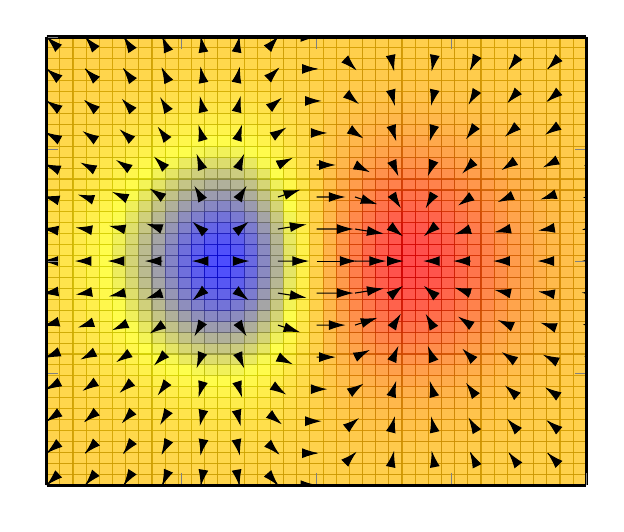
\begin{tikzpicture}
        \begin{axis}[
            domain=-2:2,
            view={0}{90},
            axis line style ={very thick},
            xmin=-2, xmax=2,
            ymin=-2, ymax=2,
            yticklabel=\empty,
            xticklabel=\empty,
          ]
          \addplot3
          [surf,
            samples=42,
            opacity=0.7,
          ]
          {x/(0.01*exp(x^2+y^2))};
          \addplot3
          [black,
          point meta={
              sqrt(
              ((1-2*x^2)*exp(-x^2-y^2))^2+
              (-2*x*y*exp(-x^2-y^2))^2
              )
            },
          quiver={
          u={(1-2*x^2)*exp(-x^2-y^2)},
          v={-2*x*y*exp(-x^2-y^2)},
          scale arrows=0.3,
          every arrow/.append style={%
          -{Latex[scale length={max(0.01,\pgfplotspointmetatransformed/400)}]},
          },
          },
          samples=15]
          {x/(0.01*exp(x^2+y^2))};
        \end{axis}
      \end{tikzpicture}
    \end{minipage}
  }
\end{figure}
\end{document}